\documentclass[11pt, a4paper]{article}

\usepackage[utf8]{inputenc}
\usepackage[T1]{fontenc}
\usepackage[english]{babel}

\usepackage{array}
\usepackage{fancybox}
\usepackage{textcomp}
\usepackage{sectionbox}

\usepackage{fancyhdr}
\usepackage{fancyvrb}
\usepackage{titletoc}
\usepackage[hyperref,html,x11names]{xcolor}
\usepackage[colorlinks=true,pdftex=true,linkcolor=SteelBlue4]{hyperref}
\usepackage{graphicx}

%% --- Maths
\usepackage{latexsym}
\usepackage{amsfonts}
\usepackage{amssymb}

%% --- Page geometry
\textwidth 16cm
\textheight 23.5cm
\headsep 1cm
\topmargin -1.5cm
\oddsidemargin 0cm
\setlength{\unitlength}{1cm}

%% --- C#
\newcommand{\csharp}{\textsc{C\#}}

%% --- FancyHDR
\pagestyle{fancy}
\lhead{
  {\textbf{\csharp}}\\
  {\textsc{tp}} 6 -- January 2014}
\rhead{
  {\small Info-Sup}\\
  {\textsc{Epita}}}
%% *** Logo
\rfoot{
\includegraphics[width=3.5cm]{../res/logo.pdf}}

%% -- Code environment (no syntax highlighting).
\newenvironment{code}%
{
\definecolor{sectboxfillcol}{rgb}{1,1,1}
\VerbatimEnvironment
\begin{center}
\framesectionbox
\small
\begin{sectionbox}[\textwidth]{}
\vspace{1mm}
\begin{Verbatim}
}%
{
\end{Verbatim}
\end{sectionbox}
\end{center}
}

%% -- XColor configuration
\hypersetup{urlcolor=cyan}

%% -- Pandoc syntax highlighting

\DefineShortVerb[commandchars=\\\{\}]{\|}
\DefineVerbatimEnvironment{Highlighting}{Verbatim}{commandchars=\\\{\}, frame=single, label=Source code, fontsize=\small}
\newenvironment{Shaded}{}{}
\newcommand{\KeywordTok}[1]{\textcolor[rgb]{0.00,0.44,0.13}{\textbf{{#1}}}}
\newcommand{\DataTypeTok}[1]{\textcolor[rgb]{0.56,0.13,0.00}{{#1}}}
\newcommand{\DecValTok}[1]{\textcolor[rgb]{0.25,0.63,0.44}{{#1}}}
\newcommand{\BaseNTok}[1]{\textcolor[rgb]{0.25,0.63,0.44}{{#1}}}
\newcommand{\FloatTok}[1]{\textcolor[rgb]{0.25,0.63,0.44}{{#1}}}
\newcommand{\CharTok}[1]{\textcolor[rgb]{0.25,0.44,0.63}{{#1}}}
\newcommand{\StringTok}[1]{\textcolor[rgb]{0.25,0.44,0.63}{{#1}}}
\newcommand{\CommentTok}[1]{\textcolor[rgb]{0.38,0.63,0.69}{\textit{{#1}}}}
\newcommand{\OtherTok}[1]{\textcolor[rgb]{0.00,0.44,0.13}{{#1}}}
\newcommand{\AlertTok}[1]{\textcolor[rgb]{1.00,0.00,0.00}{\textbf{{#1}}}}
\newcommand{\FunctionTok}[1]{\textcolor[rgb]{0.02,0.16,0.49}{{#1}}}
\newcommand{\RegionMarkerTok}[1]{{#1}}
\newcommand{\ErrorTok}[1]{\textcolor[rgb]{1.00,0.00,0.00}{\textbf{{#1}}}}
\newcommand{\NormalTok}[1]{{#1}}

\begin{document}

\begin{center}
  {\Large {\textbf{Files \& Bits}}}
\end{center}

\section{Submission}\label{submission}

Your submission \textbf{must} be a \texttt{zip} file.

\subsection{\texttt{AUTHORS} file}\label{authors-file}

This file contains your \emph{login} with the following rules: an
asterisk \texttt{*}, a space, your \emph{login} (\texttt{login\_x}) and
a newline -- which is represented by the \texttt{\$} character in the
following example:

\begin{verbatim}
    * login_x$
\end{verbatim}

\subsection{Directory tree}\label{directory-tree}

The name of the \texttt{zip} file is \texttt{rendu-tpcs6-login\_x.zip}
and follows this directory tree:

\begin{code}
    rendu-tp6-login_x.zip
        | login_x/
            | AUTHORS
            | BMPReader/
                | BMPReader/*
                | BMPReader.sln
            | DataHiding
                | DataHiding/*
                | DataHiding.sln
            | GameMap/
                | GameMap/*
                | GameMap.sln
\end{code}

\begin{itemize}
\itemsep1pt\parskip0pt\parsep0pt
\item
  The file \texttt{README} is advised in case of bonuses.
\item
  No \emph{dump} file is allowed. No \texttt{bin/} or \texttt{obj/} in
  the archive.
\item
  Do not finish this pratical at the last minute.
\item
  \textbf{The code has to compile.} Do not forget to check your archive.
\end{itemize}
\section{Introduction}\label{introduction}

This TP will cover the basics about file manipulation (\texttt{BMP}
images), and bits to do steganography.
\section{\texttt{static} keyword}\label{static-keyword}

\texttt{Static} modifier is used to declare a static member, \emph{i.e.}
refer to the \emph{type} rather than a specific object. The keyword
\texttt{static} is used with classes, fields, methods, properties,
operators, events and constructors. \newline

\begin{itemize}
\itemsep1pt\parskip0pt\parsep0pt
\item
  Designating a \emph{static class} means that all members and class
  methods are static, for example the \texttt{Convert} class does not
  need to be used with an instance.
\item
  Another example like \texttt{Console.WriteLine} means a \emph{class
  method} (or static method) that can be used without having to
  instantiate an object such as \texttt{Console}.
\item
  We can also refer to a method in a \emph{static variable}. This keeps
  the result of this variable whenever calls are made to this method.
\end{itemize}

\begin{Shaded}
\begin{Highlighting}[]
\CommentTok{/* This is useless. */}
\KeywordTok{static} \DataTypeTok{void} \FunctionTok{UpdateCount}\NormalTok{()}
\NormalTok{\{}
    \KeywordTok{static} \DataTypeTok{int} \NormalTok{count = }\DecValTok{0}\NormalTok{;}
    \NormalTok{count++;}
\NormalTok{\}}
\end{Highlighting}
\end{Shaded}

In the example, the \texttt{UpdateCount} method contains a variable of
type \texttt{int} named \texttt{count}. This variable is initialized to
zero at the first call to the \texttt{UpdateCount} method. On subsequent
calls to the \texttt{UpdateCount}, \texttt{count} variable is not worth
zero, but rather the value resulting from the preceding call.
\section{Program arguments}\label{program-arguments}

The \texttt{Main} method is the entry point of all programs.It is here
that the program begins and ends. This method has the particularity of
handling arguments of the program.

\begin{code}
program.exe arg0 arg1 arg2
\end{code}

In the above example, arguments are placed in the \emph{string} array
that is one argument of the \texttt{Main} function. You can access to
\texttt{"arg0"} by doing \texttt{args{[}0{]}}, etc \ldots{}

\begin{Shaded}
\begin{Highlighting}[]
\KeywordTok{class} \NormalTok{TestClass}
\NormalTok{\{}
    \KeywordTok{static} \KeywordTok{private} \DataTypeTok{void} \FunctionTok{Main}\NormalTok{(}\DataTypeTok{string}\NormalTok{[] args)}
    \NormalTok{\{}
        \CommentTok{/* Display the number of command line arguments. */}
        \NormalTok{System.}\FunctionTok{Console}\NormalTok{.}\FunctionTok{WriteLine}\NormalTok{(args.}\FunctionTok{Length}\NormalTok{);}
    \NormalTok{\}}
\NormalTok{\}}
\end{Highlighting}
\end{Shaded}

\begin{itemize}
\itemsep1pt\parskip0pt\parsep0pt
\item
  The \texttt{Main} method can return an integer (which is often use as
  error code). You just have to replace \texttt{void} with \texttt{int}.
\item
  If the program never takes arguments, \texttt{string{[}{]} args} is
  optional. Notice that the arguments array can take names other than
  \emph{args}.
\item
  The \texttt{Main} method must always be \texttt{private} and
  \texttt{static}.
\end{itemize}
\section{\texttt{struct} keyword --
Structures}\label{struct-keyword-structures}

Structures are used to encapsulate a small group of variables, for
example, characteristics of an object inventory.

\begin{Shaded}
\begin{Highlighting}[]
\KeywordTok{public} \KeywordTok{struct} \NormalTok{Book}
\NormalTok{\{}
    \KeywordTok{public} \DataTypeTok{decimal} \NormalTok{price;}
    \KeywordTok{public} \DataTypeTok{string} \NormalTok{title;}
    \KeywordTok{public} \DataTypeTok{string} \NormalTok{author;}
\NormalTok{\}}
\end{Highlighting}
\end{Shaded}

A structure can contain constructors, constants, fields, properties,
events, etc. But in these cases it is better to make a class.
\section{Binary files}\label{binary-files}

The files do not contain any text. A binary file (for example
\texttt{BMP}, \texttt{EXE}, \texttt{MP3}, etc.) will be unreadable in a
text editor such as \texttt{NotePad}. These files have a structure (they
are said to be \emph{formatted}) particular depending on the type. Most
binary files begin with a \emph{field} called \emph{magic number}. This
field is a signature of a few bytes to identify the file type.

For example, a \texttt{PDF} file starts with 4 bytes in \texttt{ASCII}
format: \texttt{\%PDF}. In the case of a \texttt{BMP} file, the
\emph{magic number} is \texttt{BM}.

\subsection{\texttt{BMP} file format}\label{bmp-file-format}

The \emph{bitmap} format is uncompressed image file. It is composed of 3
zones:

\begin{itemize}
\itemsep1pt\parskip0pt\parsep0pt
\item
  the header;
\item
  the color palette;
\item
  data relating to the image.\newline
\end{itemize}

Full details on the \texttt{BMP} format:
\url{http://en.wikipedia.org/wiki/BMP_file_format}

\begin{table}[h]
\begin{center}
\begin{ttfamily}
\begin{tabular}{l||l}
Field name & Size in byte \\
\hline
Magic Number & 2 \\
File Size & 4 \\
Reserved1 & 2 \\
Reserved2 & 2 \\
File Offset to PixelArray & 4 \\
DIB Header Size & 4 \\
Image Width & 4 \\
Image Height & 4 \\
Planes & 2 \\
Bits per Pixel & 2 \\
... & ...
\end{tabular}
\end{ttfamily}
\end{center}
\caption{Structure of the BMP file header.}
\end{table}

Certain information contained in the header are not useful for this
practical.\newline

To read the information contained in this header, we use the
\texttt{BinaryReader} class that can read data from a stream and store
it in a type.

\begin{Shaded}
\begin{Highlighting}[]
\CommentTok{/* Open the file. */}
\NormalTok{FileStream fs = }\KeywordTok{new} \FunctionTok{FileStream}\NormalTok{(}\StringTok{"filename.ext"}\NormalTok{, FileMode.}\FunctionTok{Open}\NormalTok{, FileAccess.}\FunctionTok{Read}\NormalTok{);}
\NormalTok{BinaryReader br = }\KeywordTok{new} \FunctionTok{BinaryReader}\NormalTok{(fs);}
\CommentTok{/* Reads an 32 bits (4 bytes) signed integer. */}
\DataTypeTok{int} \NormalTok{i = br.}\FunctionTok{ReadInt32}\NormalTok{();}
\CommentTok{/* Reads a character (1 byte). */}
\DataTypeTok{char} \NormalTok{c = br.}\FunctionTok{ReadChar}\NormalTok{();}
\NormalTok{fs.}\FunctionTok{Close}\NormalTok{();}
\end{Highlighting}
\end{Shaded}

\subsection{Read \texttt{BMP} file with
\texttt{.NET}}\label{read-bmp-file-with-.net}

\texttt{.NET} framework provided a class for editing \texttt{BMP} files.
This class is contained in the component \texttt{System.Drawing}.

\begin{Shaded}
\begin{Highlighting}[]
\KeywordTok{using} \NormalTok{System.}\FunctionTok{Drawing}\NormalTok{;}
\NormalTok{...}
\CommentTok{/* Loads a bitmap file. */}
\NormalTok{Bitmap img = }\KeywordTok{new} \FunctionTok{Bitmap}\NormalTok{(}\StringTok{"filename.bmp"}\NormalTok{);}
\end{Highlighting}
\end{Shaded}
\section{XNA Game Studio}\label{xna-game-studio}

Extract from
MSDN\footnote{\url{http://msdn.microsoft.com/en-us/library/bb203894.aspx}}:

\begin{quote}
XNA Game Studio is an integrated development environment designed to make it easier to develop games for Microsoft Windows, Xbox 360, and Windows Phone. XNA Game Studio extends Microsoft Visual Studio with support for the XNA Framework and tools. The XNA Framework is a managed-code class library that contains features targeted specifically at game development. In addition, XNA Game Studio includes tools for adding graphic and audio content to your game.
\end{quote}

Step by step documentation:
\url{http://msdn.microsoft.com/en-us/library/bb203893.aspx}

\subsection{Construction of a game}\label{construction-of-a-game}

A video game begins with an initialization phase in which images are
loaded into memory. Then the game takes place in a cycle (an infinite
loop) which successively produce the updated game elements and the
display of images.

XNA sets up place the basic mechanisms of the game. In this pratical it
is important to remember:\newline

\begin{itemize}
\itemsep1pt\parskip0pt\parsep0pt
\item
  Graphic resources are loaded in the \texttt{LoadContent} method.
\item
  Set configuration is updated in the \texttt{Update} method.
\item
  Rendering the image in the \texttt{Draw} method.\newline
\end{itemize}

\subsection{Add a \emph{sprite}}\label{add-a-sprite}

Perform a simple drag and drop of the image in the Solution Explorer in
Content Manager. Configure (\emph{Properties}) the asset name by putting
a name explaining the content of the image (if needed). Note also that
you can make settings for the transparency (designate a color filter).

\subsection{Load a \emph{sprite}}\label{load-a-sprite}

Add a \texttt{Texture2D} attribute and \texttt{Vector2} or
\texttt{Rectangle} in the \texttt{Game1} class and edit the
\texttt{LoadContent} method:

\begin{Shaded}
\begin{Highlighting}[]
\CommentTok{// This is a texture we can render.}
\NormalTok{Texture2D myTexture;}

\CommentTok{// Set the coordinates to draw the sprite at.}
\NormalTok{Vector2 spritePosition = Vector2.}\FunctionTok{Zero}\NormalTok{;}

\KeywordTok{protected} \KeywordTok{override} \DataTypeTok{void} \FunctionTok{LoadContent}\NormalTok{()}
\NormalTok{\{}
    \CommentTok{// Create a new SpriteBatch, which can be used to draw textures.}
    \NormalTok{spriteBatch = }\KeywordTok{new} \FunctionTok{SpriteBatch}\NormalTok{(GraphicsDevice);}
    \NormalTok{myTexture = Content.}\FunctionTok{Load}\NormalTok{<Texture2D>(}\StringTok{"mytexture"}\NormalTok{);}
\NormalTok{\}}
\end{Highlighting}
\end{Shaded}

\subsection{Draw a \emph{sprite}}\label{draw-a-sprite}

Edit the \texttt{Draw} method. Always specify when you start drawing and
when you have finished. The \texttt{Draw} method is called for each
\emph{frame} generation and we must \emph{clean up} the drawing surface.

\begin{Shaded}
\begin{Highlighting}[]
\KeywordTok{protected} \KeywordTok{override} \DataTypeTok{void} \FunctionTok{Draw}\NormalTok{(GameTime gameTime)}
\NormalTok{\{}
    \NormalTok{graphics.}\FunctionTok{GraphicsDevice}\NormalTok{.}\FunctionTok{Clear}\NormalTok{(Color.}\FunctionTok{CornflowerBlue}\NormalTok{);}

    \CommentTok{// Draw the sprite.}
    \NormalTok{spriteBatch.}\FunctionTok{Begin}\NormalTok{();}
    \NormalTok{spriteBatch.}\FunctionTok{Draw}\NormalTok{(myTexture, spritePosition, Color.}\FunctionTok{White}\NormalTok{);}
    \NormalTok{spriteBatch.}\FunctionTok{End}\NormalTok{();}

    \KeywordTok{base}\NormalTok{.}\FunctionTok{Draw}\NormalTok{(gameTime);}
\NormalTok{\}}
\end{Highlighting}
\end{Shaded}
\section{Exercise 1 : \texttt{BMPReader}}\label{exercise-1-bmpreader}

You have to write a program that uses, as a parameter a filename, and
prints information. \textbf{You must not use the \texttt{.NET} API in
this exercise} and you must read the file using \texttt{BinaryReader}.

\subsection{Arguments handler}\label{arguments-handler}

You have to handle the case in which the user is calling your program
with wrong arguments. The program needs only one argument.

\begin{code}
bmpreader.exe image.bmp
\end{code}

\begin{itemize}
\itemsep1pt\parskip0pt\parsep0pt
\item
  If no arguments or more than two arguments are used, display a help
  message:
\end{itemize}

\begin{code}
Error: This program needs only one argument.
Usage: bmpreader.exe <file.bmp>
\end{code}

\begin{itemize}
\itemsep1pt\parskip0pt\parsep0pt
\item
  If after checking, the file path is incorrect:
\end{itemize}

\begin{code}
Error: The file path is invalid.
Usage: bmpreader.exe <file.bmp>
\end{code}

\subsection{\emph{Magic number} checker}\label{magic-number-checker}

Before going any further, we check the \emph{magic number}. If it does
not match to a \emph{bitmap} image file, the program exits and prints an
error message:

\begin{itemize}
\itemsep1pt\parskip0pt\parsep0pt
\item
  Full file path.
\item
  Tell the user that the file is not a \texttt{BMP} file.
\end{itemize}

\begin{code}
C:\path\file.txt : This file is not an bitmap (BMP) file.
\end{code}

\subsection{Information printer}\label{information-printer}

If no error appears, you must display the following information:

\begin{itemize}
\itemsep1pt\parskip0pt\parsep0pt
\item
  Picture dimensions
\item
  Number of bits per pixel
\end{itemize}

Display information by following the example:

\begin{code}
C:\path\file.bmp file informations:
    - Magic number is valid.
    - Dimensions: 420x314
    - Number of bits per pixel: 24
\end{code}

Do not forget to put a newline character even if it is the last line.
\section{Exercise 2 : \texttt{DataHiding}}\label{exercise-2-datahiding}

The purpose of this exercise is to show you another way to transfer a
message, like the way of our good old friend 007-through steganography.

\subsection{Short History}\label{short-history}

A few weeks ago, you discovered a way to send a message in encrypted
form, thanks to cryptography. This method consisted in changing the
original message to hide it from people that don't know the private key.
This method is very useful, but not really discreet.

The idea of the steganography system is to hide a message in another
message. Steganography can be performed in the real world using ink made
from lemon juice, visible only in a hot environment. Today we will learn
how to hide a message in an image.

\subsection{Stegano in a 24-bit
bitmap}\label{stegano-in-a-24-bit-bitmap}

In the 24-bit bitmap that we will use, every pixel is represented by 24
bits. In these 24 bits, each component (red, green and blue) is coded on
8 bits.

To hide our information, we will exploit the fact that two colours that
are too close are indistinguishable for humans. We will use the last bit
of each byte to hide our data (because it is the least significant bit;
the change is to alter the byte less than 0.4\%, whereas changing the
first bit, the MSB or most significant bit, would have made for example
changed 50 to 178, which is a big difference).

Thus, if we want to hide ``5'' (101 in binary) in a pixel (240, 65,
169), in binary (11110000, 00100001, 10101011) is going to take each bit
of ``5'' and put it on less significant bit components of these pixels.
The first is a 1, so the first component takes 1 on the less significant
bit, thus becoming 241 (11110001 in binary). The second is a 0, so the
second component takes a 0 on the less significant bit, thus becoming 64
(00100000 in binary). The last is a 1, so the third component takes 1 on
the less significant bit, which changes nothing.

We will hide text. The text is nothing more than a series of ASCII
characters, which as we know, are bytes. So it takes 8 components,
meaning almost three pixels, to hide a single character.

\subsection{Let's go !}\label{lets-go}

For this exercise, you are truly free to choose your method, as you'll
soon have to stand on your own two feet !

So you have to write a program, that will allow the user to choose an
image, then load and retrieve a hidden message inside. This program will
of course have a second function, that of hiding a message in an image.
Of course, you will still need some guidance this year, we know very
well that you can't fly yet!

\subsubsection{Getting Started}\label{getting-started}

This part will show you how to make this program.

First, we recommend that you to create a Windows Form project, wich will
give you a fast interface and many possibilities for your program.

In our example, we will say that your interface has three button and a
textBox. A button to load the image, a button (named
\texttt{hideButton}) to hide the text in the textBox in a copy of the
picture called \texttt{result.bmp}, and finally a button (named
\texttt{revealButton}) to read the message hidden in the loaded image.

\subsubsection{Image , Image \ldots{} show me your
message!}\label{image-image-show-me-your-message}

Now that the interface is raised, you will code the following function
created by double clicking on the button \texttt{revealButton} :

\begin{Shaded}
\begin{Highlighting}[]
\KeywordTok{private} \DataTypeTok{void} \FunctionTok{revealButton_Click} \NormalTok{(}\DataTypeTok{object} \NormalTok{sender, EventArgs e);}
\end{Highlighting}
\end{Shaded}

This function is called when the button is clicked, so check at the
beginning of the function that the image is correctly loaded. Then you
have to browse the image line by line to get the whole message. We will
define that a message will always end with a `\textbackslash{}0' or null
character, corresponding to the character in position 0 in the
\texttt{ASCII} table.

Do not forget the loops TP, especially dual loop \texttt{for}, they will
be useful. Restore the message on the textBox.

\texttt{Tip:} the least significant bit is the parity of a number.

\subsubsection{Your mission, should you decide to accept
it}\label{your-mission-should-you-decide-to-accept-it}

We know now how to recover a hidden message. Let us see how to hide
ours.

You will code the following function created by a double click on the
button \texttt{hideButton} :

\begin{Shaded}
\begin{Highlighting}[]
\KeywordTok{private} \DataTypeTok{void} \FunctionTok{hideButton_Click} \NormalTok{(}\DataTypeTok{object} \NormalTok{sender, EventArgs e);}
\end{Highlighting}
\end{Shaded}

Again, check that an image is loaded. Then we need to get back the
message written TextBox and for each character, recover corresponding
\texttt{ASCII} code and convert it to binary. Once binarized, the
character can be inserted in the image, byte by byte. Do not forget the
`\textbackslash{}0' at the end of the message.
\section{Exercise 3 : \texttt{GameMap}}\label{exercise-3-gamemap}

In this exercise you will model a game map using the \texttt{BMP}
format. This will allow you to easily create maps without using any map
editing tool. You can go further by creating for example a map with
multiple layers:

\begin{itemize}
\itemsep1pt\parskip0pt\parsep0pt
\item
  a background layer
\item
  an event layer to make actions depending on the color (fight,
  dialogue, etc.)
\item
  an object layer to draw special objects on the map.\newline
\end{itemize}

In this exercise you must draw, the image using XNA.

\begin{figure}[h]
\begin{center}

\includegraphics[width=2cm]{../res/mapbmp.png}
\end{center}
\caption{\texttt{BMP} picture of size \texttt{10x10} representing the map.}
\end{figure}

\subsection{Preparation}\label{preparation}

Create a new XNA project named \texttt{GameMap} in Visual Studio 2010.
Then add the following component
\texttt{System.Drawing}\footnote{Beware! This component adds another refererence to the class \texttt{Color}. You will have to specify the namespace, for example: \texttt{System.Drawing.Color}.}.
In \emph{Solution explorer}, right-click on \emph{References}, \emph{Add
Reference\ldots{}} and search in \texttt{.NET}. To finish, add at the
beginning of the \texttt{Game1.cs} file:

\begin{Shaded}
\begin{Highlighting}[]
\KeywordTok{using} \NormalTok{System.}\FunctionTok{Drawing}\NormalTok{;}
\end{Highlighting}
\end{Shaded}

We will draw rectangles with \texttt{XNA}. For each drawing instruction,
\texttt{XNA} needs a \texttt{Texture2D}. Create a \texttt{BMP} picture:

\begin{itemize}
\itemsep1pt\parskip0pt\parsep0pt
\item
  File name : \texttt{blank.bmp}
\item
  Dimensions : \texttt{1x1}
\item
  Pixel color : white
\end{itemize}

Add the picture in \texttt{GameMapContent} section.\newline

Create another \texttt{BMP} picture to design the map. Add it in the
\texttt{GameMapContent} and setup VS to copy the image in the output
directory (where there is the executable) : \texttt{Properties} and
\texttt{Copy always} set to \texttt{Copy to Output Directory}.

\subsection{Implementation}\label{implementation}

Add the following fields in \texttt{Game1} class:

\begin{Shaded}
\begin{Highlighting}[]
\CommentTok{/* BMP file that contains our map. */}
\NormalTok{Bitmap map;}
\CommentTok{/* Blank texture to draw Rectangle. */}
\NormalTok{Texture2D blank;}
\end{Highlighting}
\end{Shaded}

The \texttt{BMP} picture representing the map is located in the
\texttt{Content} directory whose path is the property
\texttt{RootDirectory}:

\begin{code}
this.Content.RootDirectory + "\\map.bmp"
\end{code}

Load the \texttt{BMP} picture and the \texttt{Texture2D}
(\emph{cf.~course notes for this TP}) in this method:

\begin{Shaded}
\begin{Highlighting}[]
\KeywordTok{protected} \KeywordTok{override} \DataTypeTok{void} \FunctionTok{LoadContent}\NormalTok{();}
\end{Highlighting}
\end{Shaded}

To finish, implement the following method in \texttt{Game1} class. This
method reads the \texttt{BMP} file and draw rectangles (representing
pixels).

\begin{Shaded}
\begin{Highlighting}[]
\CommentTok{/* Draw the map on the screen. */}
\KeywordTok{private} \DataTypeTok{void} \FunctionTok{DrawMap}\NormalTok{();}
\end{Highlighting}
\end{Shaded}

\begin{itemize}
\itemsep1pt\parskip0pt\parsep0pt
\item
  Use properties \texttt{Width} and \texttt{Height} of \texttt{Bitmap}
  class.
\item
  Create instances of class \texttt{Microsoft.Xna.Framework.Color} by
  using pixel value of \texttt{System.Drawing.Color}, use properties
  \texttt{R}, \texttt{G} and \texttt{B}.
\item
  Get dimensions of \texttt{XNA}'s window:
\end{itemize}

\begin{Shaded}
\begin{Highlighting}[]
\DataTypeTok{int} \NormalTok{screen_height = }\KeywordTok{this}\NormalTok{.}\FunctionTok{GraphicsDevice}\NormalTok{.}\FunctionTok{Viewport}\NormalTok{.}\FunctionTok{Height}\NormalTok{;}
\DataTypeTok{int} \NormalTok{screen_width = }\KeywordTok{this}\NormalTok{.}\FunctionTok{GraphicsDevice}\NormalTok{.}\FunctionTok{Viewport}\NormalTok{.}\FunctionTok{Width}\NormalTok{;}
\end{Highlighting}
\end{Shaded}

Now, add three lines in this method to draw the map:

\begin{Shaded}
\begin{Highlighting}[]
\KeywordTok{protected} \KeywordTok{override} \DataTypeTok{void} \FunctionTok{Draw}\NormalTok{(GameTime gameTime);}
\end{Highlighting}
\end{Shaded}

\begin{figure}[h]
\begin{center}
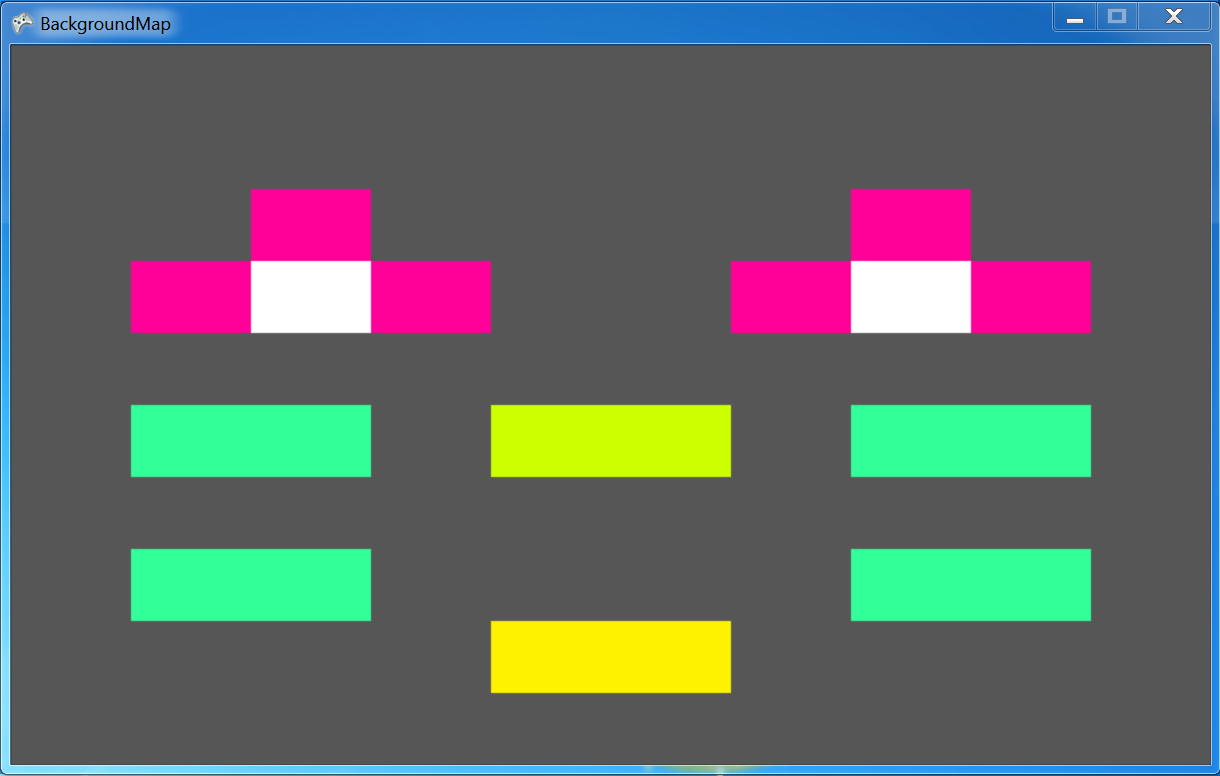
\includegraphics[width=10cm]{../res/mapxna.png}
\end{center}
\caption{Map drawing in XNA.}
\end{figure}
\end{document}
